\documentclass{scrartcl}

\usepackage{amsmath}
\usepackage{hyperref}
\usepackage[style=iso]{datetime2}
\usepackage[margin=1mm]{geometry}
\usepackage{multicol}

\usepackage{listings}
\usepackage{color}
\usepackage{tikz}
\usetikzlibrary{%
    decorations.pathreplacing,%
    decorations.pathmorphing%
}
\usepackage{graphicx}

% https://stackoverflow.com/questions/3175105/inserting-code-in-this-latex-document-with-indentation
\definecolor{dkgreen}{rgb}{0,0.6,0}
\definecolor{gray}{rgb}{0.5,0.5,0.5}
\definecolor{mauve}{rgb}{0.58,0,0.82}

\lstset{frame=tb,
  language=C++,
  aboveskip=3mm,
  belowskip=3mm,
  showstringspaces=false,
  columns=flexible,
  basicstyle={\small\ttfamily},
  numberstyle=\tiny\color{gray},
  keywordstyle=\color{blue},
  commentstyle=\color{dkgreen},
  stringstyle=\color{mauve},
  breaklines=true,
  breakatwhitespace=true,
  tabsize=2,
  numbers=left,
  stepnumber=1,
  xleftmargin=1cm,
  %linewidth=0.8\textwidth
}

%-----------------------------------------------------------------------
% https://tex.stackexchange.com/questions/44017/dot-notation-for-derivative-of-a-vector
% especially: https://tex.stackexchange.com/questions/44017/dot-notation-for-derivative-of-a-vector/44071#44071

\usepackage[T1]{fontenc}  % For correct {}s in \texttt
%\usepackage{amsmath}      % For better \dot placement
\usepackage[b]{esvect}    % For \vv
%\usepackage{tikz}         % For arrow and dots in \xvec

% --- Macro \xvec
\makeatletter
\newlength\xvec@height%
\newlength\xvec@depth%
\newlength\xvec@width%
\newcommand{\xvec}[2][]{%
  \ifmmode%
    \settoheight{\xvec@height}{$#2$}%
    \settodepth{\xvec@depth}{$#2$}%
    \settowidth{\xvec@width}{$#2$}%
  \else%
    \settoheight{\xvec@height}{#2}%
    \settodepth{\xvec@depth}{#2}%
    \settowidth{\xvec@width}{#2}%
  \fi%
  \def\xvec@arg{#1}%
  \def\xvec@dd{:}%
  \def\xvec@d{.}%
  \raisebox{.2ex}{\raisebox{\xvec@height}{\rlap{%
    \kern.05em%  (Because left edge of drawing is at .05em)
    \begin{tikzpicture}[scale=1]
    \pgfsetroundcap
    \draw (.05em,0)--(\xvec@width-.05em,0);
    \draw (\xvec@width-.05em,0)--(\xvec@width-.15em, .075em);
    \draw (\xvec@width-.05em,0)--(\xvec@width-.15em,-.075em);
    \ifx\xvec@arg\xvec@d%
      \fill(\xvec@width*.45,.5ex) circle (.5pt);%
    \else\ifx\xvec@arg\xvec@dd%
      \fill(\xvec@width*.30,.5ex) circle (.5pt);%
      \fill(\xvec@width*.65,.5ex) circle (.5pt);%
    \fi\fi%
    \end{tikzpicture}%
  }}}%
  #2%
}
\makeatother

% --- Override \vec with an invocation of \xvec.
\let\stdvec\vec
\renewcommand{\vec}[1]{\xvec[]{#1}}
% --- Define \dvec and \ddvec for dotted and double-dotted vectors.
\newcommand{\dvec}[1]{\xvec[.]{#1}}
\newcommand{\ddvec}[1]{\xvec[:]{#1}}
%--------------------------------------------------

\begin{document}
\title{Explanation for the ``Learning Rockets'' Computer Graphics project}
\subtitle{3D object rendering, gravitational simulation, basic event loop}
\author{ \textbf{Croitoru} Nicolae-Eugen}
% https://tex.stackexchange.com/questions/214404/add-affiliations-to-the-authors-name-in-the-article-class
\date{%
  ``Al. I. Cuza'' University of Iasi, Romania\\[2ex]%
  \today
}
\maketitle

\section{Introduction}
This is an explanation for the project ``Learning Rockets'', developed by the author for their Computer Graphics class. The program presents a rocket in the orbit of a massive planetary body, with the possibility for the rocket to thrust in any desired direction. It is aimed at students wanting a written explanation for the most important sections of the project.

These sections are:
\begin{itemize}
\item{ \textbf{3D object rendering} } details accelerated \textit{VBO} 3D rendering of objects stored in \textit{.obj} files.
\item{ \textbf{gravitational simulation} } explains how gravitational physical simulation can be achieved using fixed-timestep mathematical integration, using two similar methods (Euler and RK4).
\item{ \textbf{basic event loop} } shows how an interactive 3D application can react to inputs and events scanned and provided by a library.
\end{itemize}

In general, this example project is aimed at being relatively simple, highly compatible, very fast, while sacrificing flexibility for the sake of the aforementioned priorities.

The project is implemented in \textbf{C++}, using \textbf{OpenGL} for rendering and \textbf{SDL} as a multi-platform integration library (for window and rendering-context creation and event scanning).

The 3D rendering technique used is \textbf{Vertex Buffer Objects (VBOs)}; while old, it is relatively simple, as quick as modern techniques (for the current usecase) and relatively flexible (again, for the current usecase).

\section{3D Object Rendering}
\subsection{General Concept}
3D object rendering means, simply, putting 3D geometry on the screen. The main aim is generating a somewhat realistic and intuitive image.

While generating geometry dynamically, inside the program, is perfectly feasible, the tendency is to use pre-generated geometry (usually, created in a 3D modeling program, e.g. Blender), load it, and just display that inside the rendering program.

We're using \textbf{Vertex Buffer Objects}, which mean that the geometry data is loaded in the Video Card Random-Access Memory (\textbf{VRAM}). This has the main advantage of requiring very few function calls to draw extensive patches of geometry; this is the core of what ``accelerated 3D rendering'' means: involving the CPU as little as possible and just allowing the GPU to locally draw the geometry. Since each function requires CPU-level interruptions of code execution (especially system calls, and all draw calls are system calls), and the graphics port (e.g. PCI-E) has limited bandwidth, loading all of our geometry in advance on the video card, in large data buffers, and using just a few calls to draw those buffers, increases performance thousands of times (or even more). Further speed-ups, like increasing the computational power of the Video Card, will not be discussed here.

The main disadvantage of VBOs is their relative inflexibility; while we can update arbitrary sub-slices of VBOs, those updates are done by the CPU, and can cause slow-downs. At the time of writing, the preferred way to update geometry is \textit{shaders}. Initially, they were programs written in a C-like language, compiled and uploaded on the video card; the video card ran them during rendering, and their executions had the effect of modifying the colours in the resulting image; among the first uses for colour shaders was \textit{bloom}, allowing bright colours to create halos or lightshafts in a scene. Now, shaders are used to modify geometry as well, since the GPU (graphics processing unit) can run them and modify geometry locally, without interrupting (and interruptions from) the CPU.

However, shaders are quite a bit more difficult than VBOs to use and, in this program, unnecessary. They become more performant than VBOs when objects experience deformations (such as animating the movements of a 3D actor).

\subsection{3D Objects}
For storing 3D objects, \textit{.obj} files have been chosen. While most 3D object storage formats are binary, the \textit{.obj} format is ASCII, and thus, simpler to understand. A cube can be represented as:

\begin{lstlisting}[language=sh]
# www.blender.org
mtllib Cube.mtl
o Cube_Cube
v  1  1 -1
v  1 -1 -1
v -1 -1 -1
v -1  1 -1
v  1  1  1
v  1 -1  1
v -1 -1  1
v -1  1  1
vt 0 0
vt 0 1
vt 1 1
vt 1 0
vn  0  0 -1
vn  0  0  1
vn  1  0  0
vn  0 -1  0
vn -1  0  0
vn  0  1  0
usemtl CubeMtl
f 1/1/1 2/2/1 3/3/1 4/4/1 
f 5/4/2 8/3/2 7/2/2 6/1/2 
f 1/3/3 5/4/3 6/1/3 2/2/3 
f 2/4/4 6/1/4 7/2/4 3/3/4 
f 3/1/5 7/2/5 8/3/5 4/4/5 
f 5/2/6 1/3/6 4/4/6 8/1/6 
\end{lstlisting}

The first line is a comment; lines starting with \lstinline{mtllib} and \lstinline{usemtl} specify materials, which our simple renderer isn't using (materials control how light interacts with an object, such as transparency or glossiness; our objects' surfaces will look quite flat without the use of materials). The line starting with \lstinline{o} specifies the object name; for simplicity, we only parse one object per file in this program.

\subsubsection{3D Coordinates}

Lines starting with \lstinline{v} specify vertex coordinates - geometry coordinates in 3D space. Obviously, we have 8 vertices to our cube, and its edge length is $2$.

\subsubsection{Texture coordinates}

Lines starting with \lstinline{vt} specify texture coordinates; a texture is a 2D image of any aspect ratio. The first coordinate is the horizontal, the second is the vertical (usually named \textit{u} and \textit{v}, and the process named \textit{uv-mapping}). The mapping used here is very simple: we only specify the $4$ corners of the texture, so each vertex could have one of the corners of the texture, so each face of the cube could only represent the whole texture. More advanced use cases use points inside the texture.

\begin{figure}[ht!]
  \center
  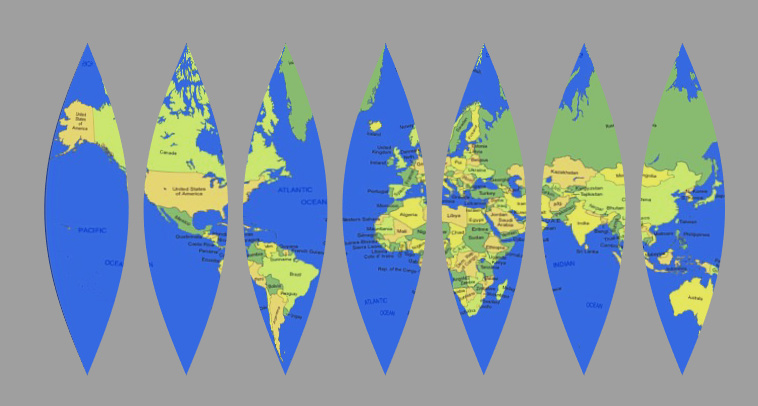
\includegraphics[width=0.5\textwidth,height=\textheight,keepaspectratio]{earthUnroll}
  \caption{A possible texture unroll for a spherical map of the Earth.\\Source: https://discourse.mcneel.com/t/unroll-3d-model-with-texture/15577}
\end{figure}

\pagebreak

\subsubsection{Normals}

Lines starting with \lstinline{vn} represent normal vectors; this means, what is the normal vector (perpendicular) to the 3D object in that point. Computer rendering use this to control light reflections: instead of defining light reflection in relation to the surface, they are defined in relation to the normal to the surface:

% http://www.texample.net/tikz/examples/oblique-incidence/
\begin{figure}[ht!]
  \center
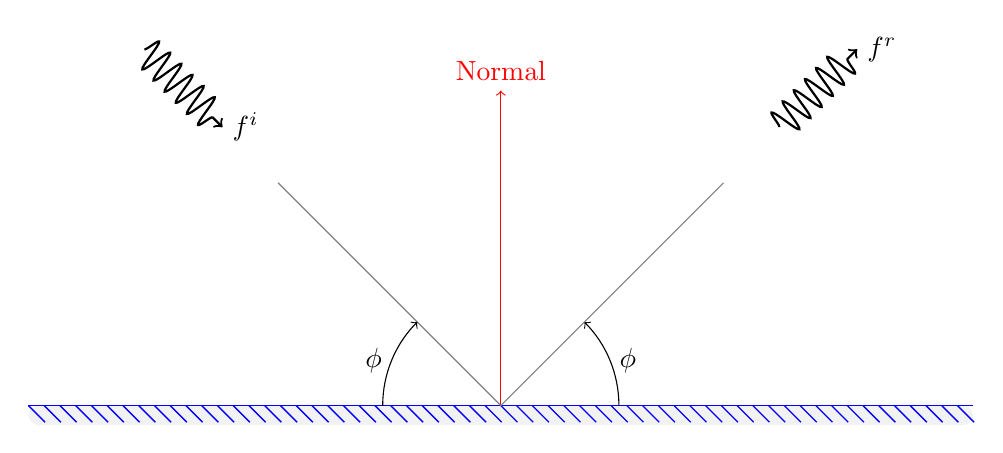
\begin{tikzpicture}[
  scale=2,
  media/.style={font={\footnotesize\sffamily}},
  wave/.style={
    decorate,decoration={snake,post length=1.4mm,amplitude=2mm,
      segment length=2mm},thick},
  interface/.style={
    % The border decoration is a path replacing decorator. 
    % For the interface style we want to draw the original path.
    % The postaction option is therefore used to ensure that the
    % border decoration is drawn *after* the original path.
    postaction={draw,decorate,decoration={border,angle=-45,
        amplitude=0.3cm,segment length=2mm}}},
  ]
  % Round rectangle
  \fill[gray!10,rounded corners] (-3,-0.125) rectangle (3,0);
  % Interface
  \draw[blue,line width=.5pt,interface](-3,0)--(3,0);
  % Vertical dashed line
  \draw[->, red](0,0)--(0,2) node[above]{Normal};
  % Incidence
  \draw[->,wave]
  (135:3.2cm)--(135:2.5cm)node[right]{$f^i$};
  \draw[gray](0:0cm)--(135:2cm);
  \draw[->](-0.75,0)arc(180:135:.75cm) node[midway, left]{$\phi$};
  \draw[->](0.75,0)arc(0:45:.75cm) node[midway, right]{$\phi$};
  % Reflection
  \draw[->,wave]
  (45:2.5cm)--(45:3.2cm)node[right]{$f^r$};
  \draw[gray](0:0cm)--(45:2cm);
\end{tikzpicture}
\caption{Reflection angles relative to surface}
\end{figure}

\begin{figure}[ht!]
  \center
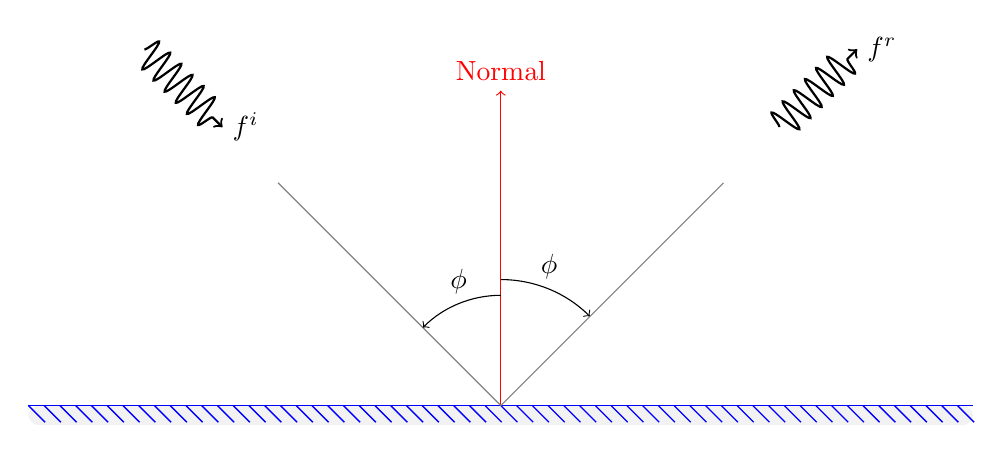
\begin{tikzpicture}[
  scale=2,
  media/.style={font={\footnotesize\sffamily}},
  wave/.style={
    decorate,decoration={snake,post length=1.4mm,amplitude=2mm,
      segment length=2mm},thick},
  interface/.style={
    % The border decoration is a path replacing decorator. 
    % For the interface style we want to draw the original path.
    % The postaction option is therefore used to ensure that the
    % border decoration is drawn *after* the original path.
    postaction={draw,decorate,decoration={border,angle=-45,
        amplitude=0.3cm,segment length=2mm}}},
  ]
  % Round rectangle
  \fill[gray!10,rounded corners] (-3,-0.125) rectangle (3,0);
  % Interface
  \draw[blue,line width=.5pt,interface](-3,0)--(3,0);
  % Vertical dashed line
  \draw[->, red](0,0)--(0,2) node[above]{Normal};
  % Incidence
  \draw[->,wave]
  (135:3.2cm)--(135:2.5cm)node[right]{$f^i$};
  \draw[gray](0:0cm)--(135:2cm);
  \draw[->](0,0.7)arc(90:135:.7cm) node[midway, above]{$\phi$};
  \draw[->](0,0.8)arc(90:45:.8cm) node[midway, above]{$\phi$};
  % Reflection
  \draw[->,wave]
  (45:2.5cm)--(45:3.2cm)node[right]{$f^r$};
  \draw[gray](0:0cm)--(45:2cm);
\end{tikzpicture}
\caption{Reflection angles relative to normal}
\end{figure}

The relative-to-normal and relative-to-surface angles are, in the above cases, an issue of notation, as both physical situations are identical.

\begin{figure}[ht!]
  \center
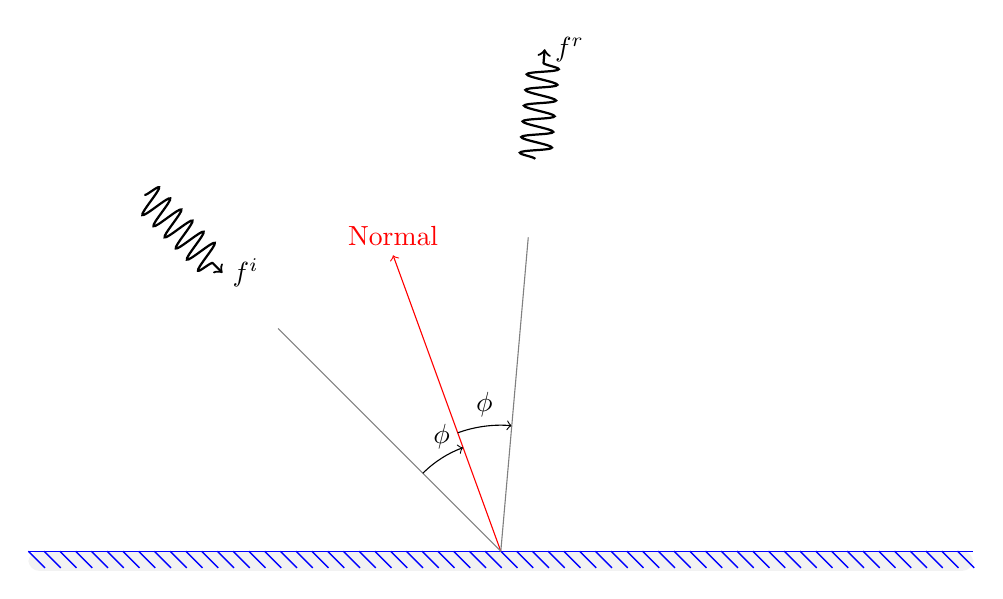
\begin{tikzpicture}[
  scale=2,
  media/.style={font={\footnotesize\sffamily}},
  wave/.style={
    decorate,decoration={snake,post length=1.4mm,amplitude=2mm,
      segment length=2mm},thick},
  interface/.style={
    % The border decoration is a path replacing decorator. 
    % For the interface style we want to draw the original path.
    % The postaction option is therefore used to ensure that the
    % border decoration is drawn *after* the original path.
    postaction={draw,decorate,decoration={border,angle=-45,
        amplitude=0.3cm,segment length=2mm}}},
  ]
  % Round rectangle
  \fill[gray!10,rounded corners] (-3,-0.125) rectangle (3,0);
  % Interface
  \draw[blue,line width=.5pt,interface](-3,0)--(3,0);
  % Vertical dashed line
  \draw[->, red](110:0)--(110:2) node[above]{Normal};
  % Incidence
  \draw[->,wave]
  (135:3.2cm)--(135:2.5cm)node[right]{$f^i$};
  \draw[gray](0:0cm)--(135:2cm);
  \draw[->](135:0.7)arc(135:110:.7cm) node[midway, above]{$\phi$};
  \draw[->](110:0.8)arc(110:85:.8cm) node[midway, above]{$\phi$};
  % Reflection
  \draw[->,wave]
  (85:2.5cm)--(85:3.2cm)node[right]{$f^r$};
  \draw[gray](0:0cm)--(85:2cm);
\end{tikzpicture}
\caption{Manipulating reflection by forcefully changing the normal}
\end{figure}

However, we can forcefully change the normal without changing the surface; this physics-incorrect way of doing reflection allows us to simulate a more complex surface by modifying light reflections, without having to model or render that detailed geometry - a trick that can yield very good looking objects that are rendered quickly.

\pagebreak

\begin{figure}[ht!]
  \center
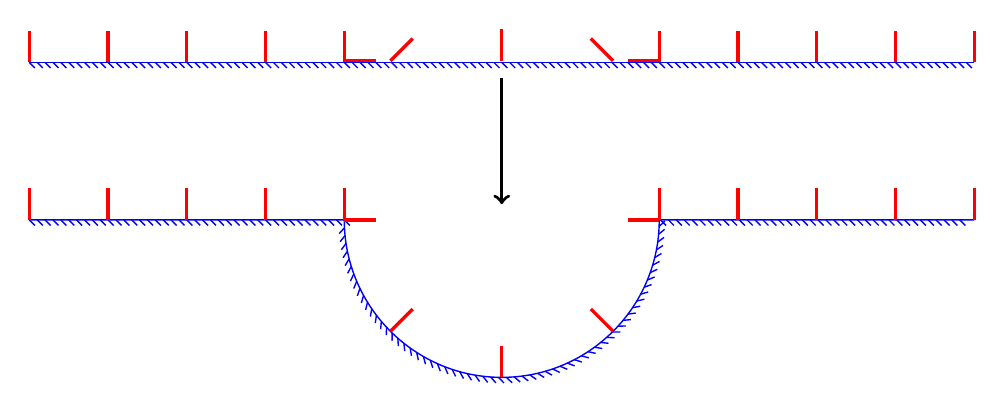
\begin{tikzpicture}[
  scale=2,
  media/.style={font={\footnotesize\sffamily}},
  interface/.style={
    % The border decoration is a path replacing decorator. 
    % For the interface style we want to draw the original path.
    % The postaction option is therefore used to ensure that the
    % border decoration is drawn *after* the original path.
    postaction={draw,decorate,decoration={border,angle=-45,
        amplitude=0.1cm,segment length=1mm}}},
  ]
  % Round rectangle
  %\fill[gray!10,rounded corners] (-3,-0.125) rectangle (3,0);
  % Interface
  \draw[->, very thick] (0, 0.9) -> (0, 0.1);
  \draw[blue,line width=.5pt,interface](-3,1) -- (3, 1);
  \foreach \ii in {-3, -2.5, ..., -1, 1, 1.5, ..., 3} {
    \draw[red, very thick](\ii, 1) -- (\ii, 1.2);
  }
  \foreach \ii in {180, 225, ..., 360} {
    \draw[red, very thick]({cos(\ii)}, 1.01) -> +({-0.2 * cos(\ii)}, {-0.2 * sin(\ii)});
  }

  \draw[blue,line width=.5pt,interface](-3,0) -- (-1,0) arc(180:360:1) -- (3, 0);
  \foreach \ii in {-3, -2.5, ..., -1, 1, 1.5, ..., 3} {
    \draw[red, very thick](\ii, 0) -- (\ii, 0.2);
  }
  \foreach \ii in {180, 225, ..., 360} {
    \draw[red, very thick](\ii:1) -- (\ii:0.8);
  }
\end{tikzpicture}
\caption{``Baking in'' normals to simplify the geometry}
\end{figure}

\subsubsection{Faces}

Lines starting with \lstinline{f} define faces. Faces are polygons; since our object is a cube, each face is a quad. Therefore, each face is made up of $4$ elements. Each element is made up of 3 references, in order: vertex, texture coordinate, normal.

Therefore, \lstinline{1/1/1} points to the first vertex, first texture coordinate and first normal defined for the object:

$(1, 1, -1) / (0, 0) / (0, 0, -1)$.

\subsection{Loading 3D objects}
\subsubsection{Parsing .obj files}

Since the \textit{.obj} format is so simple, our parser is also very simple.

\lstinline{src/objLoader.cpp}
\begin{lstlisting}
void ObjLoader::parse(ifstream* file) {
  string line, tok;
  StringVect tokens;
  while(*file != NULL) {
    getline(*file, line);
    tokens = tokenise(line);
    if(tokens.size() > 0) {
      if(tokens[0] == "v") {
        parseVertices(tokens);
      }
      else if(tokens[0] == "vt") {
        parseTexture(tokens);
      }
      else if(tokens[0] == "vn") {
        parseNormals(tokens);
      }
      else if(tokens[0] == "f") {
        parseFaces(tokens);
      } 
    }
  }
}
\end{lstlisting}

We simply split each line into tokens (by whitespace), and process vertex, texture, normal and face lines. From a simple case like vertex loading, where we simply cast the strings to float and append them to a vertex vector:

\lstinline{src/objLoader.cpp}
\begin{lstlisting}
void ObjLoader::parseVertices(StringVect tokens) {
  if(tokens.size() != 4) {
    throw(string("Error: a vertex definition should contain 3 coordinates."));
  }
  for(int i = 1; i < 4; ++i)
  m_vertices.push_back(::atof(tokens[i].c_str()));
}
\end{lstlisting}

to a more intricate case, where we parse a number of different kinds of faces: when an object has 3D coordinates, texture coordinates and normal coordinates, when it has only 3D coordinates and texture coordinates, and when it only has 3D coordinates:

\pagebreak

\lstinline{src/objLoader.cpp}
\begin{lstlisting}
void ObjLoader::parseFaces(StringVect tokens) {
  //we assume a very, very simple, regular object. Such object has faces consisting of a constant number of vertices.
  StringVect::iterator it, end;
  StringVect results;
  m_verticesPerFace = tokens.size() - 1;
  it = tokens.begin() + 1; //skip "f"
  end = tokens.end();
  if(m_hasUv) {
    if(m_hasNormals) {
      // f 1/1/1 2/2/1 3/3/1 4/4/1
      //   v1/vt1/vn1 ... so on
      // we change this to start at 0, such as: 1/1/1->0/0/0
      for(; it != end; ++it) {
        results = tokenise(*it, "/");
        for(int i = 0; i < 3; ++i)
        m_faces.push_back(::atoi(results[i].c_str()) - 1);
      }
    }
    else {
      // f 1/1 2/2 3/3 4/4
      //   v1/vt1 v2/vt2 ... so on
      for(; it != end; ++it) {
        results = tokenise(*it, "/");
        for(int i = 0; i < 2; ++i)
        m_faces.push_back(::atoi(results[i].c_str()) - 1);
      }
    }
  }
  else {
    //f 1 2 3 4
    for(; it != end; ++it)
    m_faces.push_back(::atof(it->c_str()));
  }
}
\end{lstlisting}

\subsubsection{Loading textures}

Textures are different from 3D objects; for a simple reason why, imagine we have 2 cubes, one red and one blue; we'd like to use the same 3D object, but apply two different textures to it.

We use the SDL library to load the bitmap textures; the data array resides in the \lstinline{.pixels} member.

The basic mechanism of loading data to memory is used throughout this OpenGL program.
\begin{enumerate}
\item We allocate a buffer for the data: \lstinline{glGenTextures(1, &texId)} allocates $1$ texture buffer, and assigns \lstinline{texId} the integer pointer to that buffer.
\item We bind the pointer as the currently active texture pointer: \lstinline{glBindTexture(GL_TEXTURE_2D, texId)}.
\item We copy the texture data, specifying the data format with: \lstinline{glTexImage2D(GL_TEXTURE_2D, 0, 3, texSdl->w, texSdl->h, 0, GL_BGR, GL_UNSIGNED_BYTE, texSdl->pixels)}. The parameters mean:
  \begin{itemize}
  \item \lstinline{GL_TEXTURE_2D}: The type of texture; this is the basic type, a 2D texture meant to be displayed.
  \item \lstinline{0}: This means the mipmap level this texture represents. When objects are viewed from far away, we can preload smaller textures (a mipmap level of 1 would be the same image, only linearly twice as small, $4$ times as small in size).
  \item \lstinline{3}: How many colours does each pixel have.
  \item \lstinline{texSdl->w}, \lstinline{texSdl->h}: width and height.
  \item \lstinline{0}: Texture border. In all versions of OpenGL, this value must be $0$.
  \item \lstinline{GL_BGR}: Colour format. We're using a Blue, Green, Red colour order.
  \item \lstinline{GL_UNSIGNED_BYTE}: The data type used to store pixels.
  \item \lstinline{texSdl->pixels}: The data array in memory. We use the array SDL allocated when loading the texture.
  \end{itemize}
\item \lstinline{glTexParameteri}: We additionally specify texture-filtering parameters (how should pixel values be interpolated if we're viewing the texture from up-close, and OpenGL has to draw more detail than is actually stored in the texture. Linear means linear interpolation.
\item \lstinline{SDL_FreeSurface(texSdl)}: The texture information is now in the VRAM. We can safely delete it from RAM, and we instruct SDL to do so.
\item \lstinline{m_tex.push_back(texId)}: We only need to remember the pointer OpenGL allocated for the texture.
\item \lstinline{m_textureMap.insert(std::pair<std::string, unsigned int>(texturePath, i))}: Additionally, we store the file path and the VRAM buffer pointer in an associative container; if we try to load the same texture twice, the second time we can skip the file loading and just return the previous pointer, thus saving VRAM space and time.
\end{enumerate}

\lstinline{src/oglDataCache.cpp}
\begin{lstlisting}
unsigned int OglDataCache::loadGlTexture(std::string texturePath) {
  SDL_Surface *texSdl = NULL;
  std::map<std::string, unsigned int>::iterator it;
  unsigned int i = 0;
  //we load all the resources at the start, and do not allow on-line modifications
  if(m_textureMap.count(texturePath) > 0) {//have we loaded this texture already?
    it = m_textureMap.find(texturePath);
    i = it->second;
  }
  //if SDL loads the texture
  else if((texSdl = SDL_LoadBMP(texturePath.c_str()))) {
    GLuint texId = 0;
    //create space for the texture, let OpenGL return its 'pointer', or Id
    glGenTextures(1, &texId);
    //set the created texture as the active texture
    glBindTexture(GL_TEXTURE_2D, texId);
    //fill the active texture from the sdl data
    glTexImage2D(GL_TEXTURE_2D, 0, 3, texSdl->w, texSdl->h, 0, GL_BGR, GL_UNSIGNED_BYTE, texSdl->pixels);
    //TexParameter are set for each texture. Do not set them globally, such as in init()
    //how should a pixel be computed when the on-screen rendered texture is smaller than the initial bitmap?
    glTexParameteri(GL_TEXTURE_2D, GL_TEXTURE_MIN_FILTER, GL_LINEAR);
    //how should a pixel be computed when the on-screen rendered texture is bigger
    glTexParameteri(GL_TEXTURE_2D, GL_TEXTURE_MAG_FILTER, GL_LINEAR);

    //we have finished generating the OpenGL texture; we can now delete the SDL texture;
    if(texSdl) {
      SDL_FreeSurface(texSdl);
      texSdl = NULL;
    }
    i = m_tex.size();
    m_tex.push_back(texId);
    //we record the position of the texture index in its vector, not its value
    m_textureMap.insert(std::pair<std::string, unsigned int>(texturePath, i));
  }
  return i;
}

\end{lstlisting}


\subsubsection{Dereferencing faces}
Since face definitions contain references, we want to replace each reference with the actual information (be it 3D coordinates, texture coordinates or normal vectors):

\lstinline{src/oglDataCache.cpp}
\begin{lstlisting}
std::vector<GLfloat> vert, tex, norm;
//face vector iterators
std::vector<GLuint>::iterator fIt, fEnd;
fIt = o.m_faces.begin();
fEnd = o.m_faces.end();
while(fIt != fEnd) {
  i = *fIt * 3;
  vert.push_back(o.m_vertices[i]);
  vert.push_back(o.m_vertices[i + 1]);
  vert.push_back(o.m_vertices[i + 2]);
  
  //texture only has U, V coordinates
  ++fIt; i = *fIt * 2;
  tex.push_back(o.m_texture[i]);
  tex.push_back(o.m_texture[i + 1]);
  
  ++fIt; i = *fIt * 3;
  norm.push_back(o.m_normals[i]);
  norm.push_back(o.m_normals[i + 1]);
  norm.push_back(o.m_normals[i + 2]);
  ++fIt;      
}
vn = vert.size() / 3; // each vertex has 3 coordinates
vArraySize = sizeof(GLfloat) * vert.size();
tArraySize = sizeof(GLfloat) * tex.size();
nArraySize = sizeof(GLfloat) * norm.size();
\end{lstlisting}

Here, we iterate through the face vector and, for each type of reference, we look it up in the appropriate vector (vetices, texture or normals) and create the three dereferenced vectors, vert, tex, norm.

\subsubsection{Loading objects to VRAM, through VBOs}

After we've dereferenced faces, we proceed to load the information to VRAM, in a process similar to texture loading. For example, to load vertices:

\begin{enumerate}
\item \lstinline{glGenBuffers(1, &vId)}: We allocate a VRAM buffer.
\item \lstinline{glBindBuffer(target, vId)}: We set that as the active buffer (all OpenGL pointer offsets now are relative to the start of the bound buffer). \lstinline{target} is \lstinline{GL_ARRAY_BUFFER}, meaning the internal structure of the data is an array.
\item \lstinline{glBufferData(target, vArraySize, &(vert[0]), usage)}: We copy the data from the vector \lstinline{vert}, to VRAM. \lstinline{vArraySize} is the size of the array, while \lstinline{usage} is \lstinline{GL_STATIC_DRAW}. This is a hint for OpenGL, promising that, mostly, we'll change the data rarely, and we'll read it (to draw it) very often. This allows OpenGL to optimise its placement within VRAM.
\item \lstinline{glGetBufferParameteriv(target, GL_BUFFER_SIZE, &vBufferSize)}: The above $3$ steps are enough to load the data. However, we want to check it has been properly uploaded to VRAM. So, we read the size of the VRAM buffer.
\item \lstinline{glDeleteBuffers(1, &vId)}: If the VRAM buffer size is incorrect, an error must have happened, such as exceeding VRAM memory. We must delete the VRAM buffer, and, probably, exit the program.
\end{enumerate}

Texture coordinate and normal loading is very similar.

\lstinline{src/oglDataCache.cpp}
\begin{lstlisting}
  GLuint vId = 0, nId = 0, tId = 0, vn;
  unsigned int vpf = o.m_verticesPerFace;//we assume a constant number of vertices per face (3 or 4)
  unsigned int target = GL_ARRAY_BUFFER, usage = GL_STATIC_DRAW;//our VBO is stored as an array. Also, it's not modified after load, merely drawn a large number of times. As such, OpenGL will likely decide to uploaded to VRAM.
  GLint vArraySize, vBufferSize = 0, nArraySize, nBufferSize = 0, tArraySize, tBufferSize = 0;//checking buffer sizes after upload, to ensure no transfer/memory problems occured.
  std::vector<GLfloat> vert, tex, norm;
  vn = vert.size() / 3; // each vertex has 3 coordinates
  vArraySize = sizeof(GLfloat) * vert.size();
  tArraySize = sizeof(GLfloat) * tex.size();
  nArraySize = sizeof(GLfloat) * norm.size();
  //VBO: create the vertex buffer object
  glGenBuffers(1, &vId);
  if(!vId) {
    cerr << "Error generating vertex buffer for " << objPath << endl;
    exit(1);
  }
  //VBO: specify the buffer type, intended usage and start and length; std::vector is guaranteed to store its information contiguously
  glBindBuffer(target, vId);
  glBufferData(target, vArraySize, &(vert[0]), usage);
  //VBO: get information about a buffer
  glGetBufferParameteriv(target, GL_BUFFER_SIZE, &vBufferSize);
  if(vArraySize != vBufferSize) {
    //VBO: always! delete buffers. They reside on the video card, and the kernel cannot clean up memory there.
    //VBO: delete a buffer identified by its Id
    glDeleteBuffers(1, &vId);
    vId = 0;
    cerr << "Error. vertex coord VBO buffer size mismatched vs. initial size. File: " << objPath << endl;
    exit(1);
  }
  
  //VBO: create the texture coord buffer object
  glGenBuffers(1, &tId);
  if(!tId) {
    cerr << "Error generating texture coord buffer for " << objPath << endl;
    exit(1);
  }
  //VBO: upload texture coordinates the same way, like vertices
  glBindBuffer(target, tId);
  glBufferData(target, tArraySize, &(tex[0]), usage);
  glGetBufferParameteriv(target, GL_BUFFER_SIZE, &tBufferSize);
  if(tArraySize != tBufferSize) {
    glDeleteBuffers(1, &tId);
    tId = 0;
    cerr << "Error. texture coord VBO buffer size mismatched vs. initial size. File: " << objPath << endl;
    exit(1);
  }
  
  //VBO: create the normals buffer object
  glGenBuffers(1, &nId);
  if(!nId) {
    cerr << "Error generating normals buffer for " << objPath << endl;
    exit(1);
  }
  //VBO: upload normals the same way
  glBindBuffer(target, nId);
  glBufferData(target, nArraySize, &(norm[0]), usage);
  glGetBufferParameteriv(target, GL_BUFFER_SIZE, &nBufferSize);
  if(nArraySize != nBufferSize) {
    glDeleteBuffers(1, &nId);
    nId = 0;
    cerr << "Error. texture coord VBO buffer size mismatched vs. initial size. File: " << objPath << endl;
    exit(1);
  }
}

\end{lstlisting}

\subsection{Rendering VBOs}
Having loaded our data to VRAM, rendering objects is mostly an issue of pointing OpenGL to the buffers and telling it to draw them.

\begin{enumerate}
\item \lstinline{glEnableClientState(GL_VERTEX_ARRAY)}: We tell OpenGL we'll be drawing vertices, from a vertex array. While we must use vertex information for a valid draw, we can dispense with other kinds of information, such as normals.
\item \lstinline{glBindBuffer(target, d.vId)}: We bind the VRAM pointer to the vertex buffer as the currently active buffer.
\item \lstinline{glVertexPointer(3, GL_FLOAT, 0, NULL)}: OpenGL needs to know the structure of the data inside the array:
  \begin{itemize}
  \item \lstinline{3}: The number of components each vertex has. Since we're drawing 3D geometry (not 2D), each vertex has 3 dimensions.
  \item \lstinline{GL_FLOAT}: The data type for each dimension.
  \item \lstinline{0}: How much space is between successive vertices. Non-$0$ values are used when interleaving vertex data with e.g. texture coord data and normal data. This technique allows the video card to draw more quickly, since most information relevant to a point is local, and this minimises video card cache misses. This would be an added layer of code complexity and, for simplicity, we haven't implemented this optimisation.
  \item \lstinline{NULL}: The offset from whence the relevant data starts (from the start of the currently bound buffer). Again, a feature used in data interleaving. 
  \end{itemize}
\item \lstinline{glBindTexture(GL_TEXTURE_2D, d.tdId)}: While normal and texture coordinate information is provided in a similar way to vertices, the texture itself must also be bound. This simple line tells OpenGL which texture to draw.
\item \lstinline{glDrawArrays(primitiveType, 0, d.vn)}: This is where the drawing happens; after we've provided OpenGL with all the necessary information to draw the object, and since that data is already in VRAM, a single function call instructs the video card to draw the object. Most of the speed of accelerated rendering is provided by this avoidance of CPU involvement in the bulk of the drawing process. The glDrawArrays function is, otherwise, equivalent to a \lstinline{glBegin(primitiveType)} instruction, containing a for-loop, which would iterate through the data arrays, from the $0$-th element up to \lstinline{d.vn}.
\item \lstinline{glDisableClientState(GL_VERTEX_ARRAY); glBindBuffer(target, 0);}: these acre clean-up instructions, disabling the features we've previously enabled in the global OpenGL state machine, and unbinding the buffer.
  
  
\end{enumerate}


\lstinline{src/oglDataCache.cpp}
\begin{lstlisting}
  void OglDataCache::renderObject(DataObject d) {
  //VBO: having the IDs of all the needed buffers, draw the object
  GLuint target = GL_ARRAY_BUFFER;
  GLuint primitiveType;
  //we decide what primitive to draw, depending on the number of vertices per face
  if(d.vpf == 3)
    primitiveType = GL_TRIANGLES;
  else if(d.vpf == 4)
    primitiveType = GL_QUADS;
  else
    primitiveType = GL_LINE_LOOP; //fallback. strange case, and we decide to just draw wireframe
  //VBO: signal tha we will be using vertex information.
  glEnableClientState(GL_VERTEX_ARRAY);
  //VBO: bind the appropriate vertex buffer; this means that pointer operations in OpenGL will be relative to the start of this buffer
  glBindBuffer(target, d.vId);
  //VBO: each vertex has 3 coordinates, is of the type GLfloat; the vertex position-related values have 0 bytes of non-related data between them (often used to interleave position, texture and normals data in the same vicinity), and the vertex position-related data starts at the very start of the buffer (offset NULL)
  glVertexPointer(3, GL_FLOAT, 0, NULL);

  //VBO: bind the texture coordinate array
  glEnableClientState(GL_TEXTURE_COORD_ARRAY);
  //VBO: also bind the appropriate texture, where the actual image resides
  glBindTexture(GL_TEXTURE_2D, d.tdId);
  glBindBuffer(target, d.tId);
  //VBO: a vertex has 2 texture coordinates 
  glTexCoordPointer(2, GL_FLOAT, 0, NULL);

  glEnableClientState(GL_NORMAL_ARRAY);
  glBindBuffer(target, d.nId);
  glNormalPointer(GL_FLOAT, 0, NULL);
  //VBO: how to draw objects where vertices are NOT shared between faces. It draws the chosen primitive type, starts with the first vertex, and ends after drawing vn vertices
  glDrawArrays(primitiveType, 0, d.vn);

  //VBO: disable the capabilities we have used
  glDisableClientState(GL_VERTEX_ARRAY);
  glDisableClientState(GL_TEXTURE_COORD_ARRAY);
  glDisableClientState(GL_NORMAL_ARRAY);
  //and unbind the buffer
  glBindBuffer(target, 0);
}
\end{lstlisting}

\subsection{Rendering the scene}

Of course, rendering objects using the above-method alone would just place those objects in the middle of the screen - or wherever their vertices are placed in the .obj file - without the possibility of placing them where and how we want. Rendering a scene means placing those objects in relationship to each other, to present a visually intelligible image.

This means, mostly translating, scaling and rotating the object in the way computed by the simulation (adjusting for the default properties of the object).
Once a proper transformation matrix has been created, we render the object using the above-method, and the object drawn will be influenced by the tranformation matrix.

Since object-specific transformations do not apply to other objects, we use the matrix stack to save and restore the basic matrix between each object draw.

\lstinline{src/engine.cpp}
\begin{lstlisting}
void Engine::render() {
  Vector3 tv; //temp vector
  Float tf; //temp float
  std::vector< SceneObject >::iterator it, end;
  while(it != end) {
    //since these are local to each object, we save and restore the modelview matrix after we're done
    glPushMatrix();

    //set object position
    tv = it->getPosition();
    glTranslatef(tv.getX(), tv.getY(), tv.getZ());

    //set object in-plane 'physics' rotation
    tf = it->getRotation() * 180.0 / M_PI; //OpenGL has degree-based angles; we use pi-radian angles in our math, but degree-based in gl-related tasks. O_o
    glRotatef(tf, 0, 0, 1); //rotation in the plane of the screen

    //apply glRotation, the correction added to the model
    tf = it->getGlRotationAngle();
    tv = it->getGlRotationAxis();
    glRotatef(tf, tv.getX(), tv.getY(), tv.getZ()); 

    //set object visual scale. It involves object size and the model scale adjustment
    tf = it->getSize(); //we do apply object visual scale adjustment here
    tf *= it->getGlScale().getX();//uniformous scale
    glScalef(tf, tf, tf);

    //this wrapper set up the modelview matrix. Now, we call the actual 'drawing' function
    renderObject(it->getDataObject());
    ++it;
    glPopMatrix(); //the transformations in this block are local to the current object
  }
}
\end{lstlisting}

There are other rendering aspects not presented here, such as 2D UI rendering on top of the 3D scene, enabling light, they are either simple enough or similar enough to the topics explained here, and adding more explanations would have distracted from this core explanation of how basic, accelerated 3D rendering can be implemented in OpenGL.

\section{Gravitational Simulation}
We implement general fixed-timestep integration to simulate motion (translation, not rotation). Simulating gravity simply means computing the forces between objects according to (Newtonian) gravity.

\subsection{Gravitational interaction}

Here, we compute all the forces between objects (this could have easily be done in a triangluar-matrix way). Additionally, we can apply non-gravitational, thrust forces for our rocket. After the forces have been properly added and the resultant force computed, we can integrate the motion.

\lstinline{src/scene.cpp}
\begin{lstlisting}
void Scene::updatePhysics(bool thrusting) {
  vector< SceneObject >::iterator begin, end, ii, jj;
  begin = m_objects.begin();
  end = m_objects.end();
  //we compute all the resultants, then accelerate and move the objects, so that objects stay still while we compute their forces
  for(ii = begin; ii != end; ++ii) {
    ii->setForce();//null resultant force
    for(jj = begin; jj != ii; ++jj) {
      ii->addForce(gravity(*ii, *jj));
    }
    for(jj = ii + 1; jj != end; ++jj) {
      ii->addForce(gravity(*ii, *jj));
    }
    //since we're iterating over our objects, we can thrust now. Ideally, we'd have a vector<bool> indicating which object is thrusting and which isn't. in the case of multiple thrusters, with multiple settings, it would be a vector< vector<Float> >. Still, this simplest case is proof of concept enough. 
    if(thrusting)
      ii->applyThrust();
  }
  //compute now, _after_ we have gotten the forces for all objects involved
  for(ii = begin; ii!= end; ++ii) {
    ii->integrate(m_dt);
  }
  updateRotation();
}
\end{lstlisting}

\subsection{Motion integration}
\subsubsection{Derivation}
In order to simulate the position of a point object in space, taking gravity into account, we need its mass, its position and its speed. As we have the masses and positions of all objects, we can compute the forces acting on them:
$$ F_g = \frac{m_1 \cdot m_2} { (r_2 - r _1)^2}$$
although establishing direction is a bit more involved.

From resultant force and mass, we can compute the total acceleration acting on a body at a point in time:
$$ \vec{F} = m \cdot \vec{a} \implies \vec{a} = \frac{\vec{F}}{m}$$

Therefore, we only need to know the position, velocity and acceleration of an object in order to predict its motion. These physical quantities are, however, connected. Let $r$ be the position of an object; its velocity $v$, is the derivative of position relative to time: it is the rate of change of position, in time. Assuming we record the position of an object at two moments, the average speed is:

$$\vec{v} = \frac{\vec{r_1} - \vec{r_0}}{t_1 - t_0}$$

If those two moments are not too far away (in time), we have $\left| t_1 - t_0 \right| < \varepsilon$, and we can reasonably assume that we've computed the instantaneous speed:
\begin{equation*}
  \left\{
    \begin{aligned}
      & \vec{v} = \frac{\vec{r_1} - \vec{r_0}}{t_1 - t_0} \\
      & \left| t_1 - t_0 \right| < \varepsilon
    \end{aligned}
  \right.
  \implies \vec{v} = \frac{d\vec{r}}{dt}
\end{equation*}

Of course, the instantaneous speed, the instantaneous rate of change, is the derivative. Thus, the velocity is the derivative of position, with respect to time.

The rate of change of velocity, with respect to time, is the acceleration.

$$ \vec{a} = \frac{d\vec{v}}{dt} = \frac{d}{dt} \cdot \frac{d\vec{r}}{dt} = \frac{dd\vec{r}}{dt^2} = \frac{d^2\vec{r}}{dt^2}$$

A standard - and handy - way of writing time-derivatives in Physics (and only time-derivatives) is the dot-notation. One dot above a quantity means its derivative with respect to time, two dots above mean its second derivative with respect to time, so on.

\begin{equation*}
  \begin{aligned}
    & \vec{v} = \frac{d\vec{r}}{dt} = \xvec[.]r \\
    & \vec{a} = \frac{d^2\vec{r}}{dt^2} = \frac{d\xvec[.]r}{dt} = \xvec[.]v = \xvec[:]r
  \end{aligned}
\end{equation*}

\subsubsection{Integration}
As stated above, we have $3$ physical quantities from which we want to predict the motion of an object: position, velocity and acceleration, $\vec r, \xvec[.]r, \xvec[:]r$.

As we have the old position and speed, and we get the new acceleration, we want to compute the influence of the new acceleration on the position and speed of the object. Velocity is the derivative of position, and acceleration is the derivative of velocity. Trying to obtain velocity from acceleration, and position from velocity means reversing the process, \textit{integrating}.

\pagebreak

Since derivation is, at least for our simple purpose, a division with a small-enough timestep, integration will be a multiplication with a small-enough timestep. Simply:

$$ \xvec[.]r = \frac{dr}{dt} \implies r = \xvec[.]r \cdot dt \; \footnote{Incorrect, since we're missing $+c$, used only for explaining}$$

Since $\xvec[.]r$ is only the rate of change, it doesn't record the starting position. Therefore, the future position will be the old position plus the rate of change in time, multiplied by time:

$$ \xvec[.]r = \frac{d\vec r}{dt} \implies \vec r = \int \xvec[.]r dt = \int \frac{d\vec r}{dt} \cdot dt = d\vec r + \vec c$$

Of course, if we have the starting position, then $\vec c = \vec r_0$, so
$ \vec r = d\vec r + \vec r_0$
and since $d\vec r = \vec r_1 - \vec r_0$, this relation checks out: $ \vec r = \vec r_1 - \vec r_0 - \vec r_0 \implies \vec r = \vec r_1$. Thus, our estimate for position should be correct (of course, $\vec r_1$ is not know, only estimated from $r_0$ and $\xvec[.]r$).

The same process is applied when integrating the acceleration to compute the current velocity $\xvec[.]r_1$:

$$ \xvec[.]r_1 = \int \xvec[:]r dt + \xvec[.]r_0 $$

Thus, the full formula is:

$$ \vec r_1 = \vec r_0 + \int \xvec[.]r dt + ( \xvec[.]r_0 + \int \xvec[:]r dt ) \cdot dt =   \vec r_0 + \int \xvec[.]r dt + \xvec[.]r_0 dt+ \int \xvec[:]r dt^2 $$

Since $dt = t_1 - t_0$, our numerical formula will be:
$$ \vec r_1 =  \vec r_0 + \int_{t_0}^{t_1} \xvec[.]r dt + \xvec[.]r_0 dt+ \int_{t_0}^{t_1} \xvec[:]r dt^2 $$

Integrating yields:

$$ \vec r_1 =  \vec r_0 + \xvec[.]r \cdot dt + \xvec[.]r_0 \cdot dt+  \frac{1}{2} \xvec[:]r \cdot dt^2 $$

A short explanation for the $\frac{1}{2}$, beyond $dx^2 = 2x$:

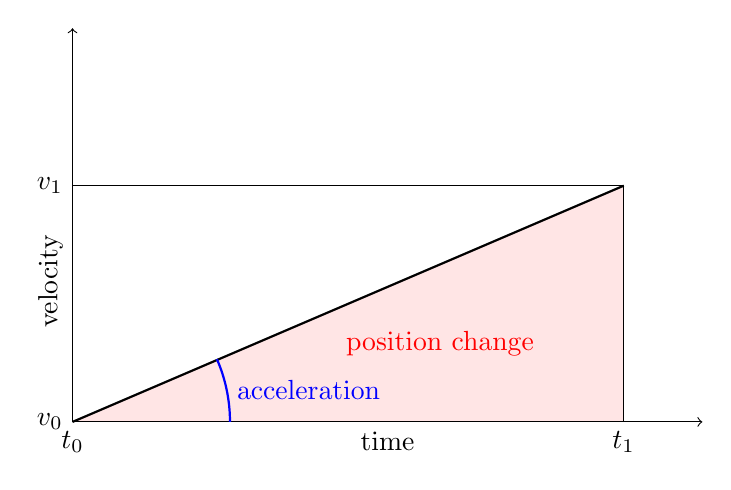
\begin{tikzpicture}
  \coordinate (p0) at (0, 0);
  \coordinate (p1) at (7, 3);
  \coordinate (p2) at (0, 3);
  \coordinate (p3) at (7, 0);
  \draw[->] (0, 0) node[left]{$v_0$} -- (0, 5) node[rotate=90, above left, midway]{velocity};
  \draw[->] (0, 0) node[below]{$t_0$} -- (8, 0) node[below, midway]{time};
  \draw(p2) node[left]{$v_1$} -- (p1) -- (p3) node[below]{$t_1$};
  \draw[fill=red!10!white](p0) -- (p3) -- (p1);
  \draw(barycentric cs:p0=1,p3=1,p1=1) node[red]{position change};
  \draw[thick](p0) -- (p1);
  \draw[blue, thick] (2, 0) arc(0:23.5:2) node[midway, right]{acceleration};
\end{tikzpicture}

If we plot position change under constant acceleration (using the dimensions velocity and time), since velocity doesn't instantly reach the final velocity, but instead gradually climbs, we can't use the square, but rather, half of the square. That's the geometric visualisation of why we use $\frac{1}{2}$.

Additionally, we can point out the geometrical interpretations of derivatives and integrals: since our dimensions are velocity and time, the derivative of velocity with respect to time is the acceleration - the slope of out line. The integral of velocity with respect to time is the surface between the line and the time axis, the triangle.

\subsubsection{Implementation}
By properly separating our full formula, we can write simpler code. Using two struct variables, one recording an object's state (its position $\vec r_0$ and velocity $\xvec[.]r_0$), another recording its state's derivative (its velocity $\xvec[.]r_1$ and acceleration $\xvec[:]r_1$), we can evaluate our integral. Of course, there are two versions for the state, the past and predicted versions. Let the past state be s for the past state, n for the new state, and d for the derivative,. Our additional inputs are the force acting on the object, from which we compute the acceleration, and $dt$. We could write:

\begin{lstlisting}
void SceneObject::eval(State s, Float dt, Vector3 force) const {
  State n;
  Derivative d;
  
  d.dv = force / self.mass; //the instant total acceleration is equal to the instant total force divided by mass
  n.v = s.v + d.dv * dt;
  
  d.dr = n.v; //obviously, since dr/t is the velocity
  n.r = s.r + d.dr * dt;
}
\end{lstlisting}

The fact that we compute the change in velocity before we update the position is important; this is called the semi-implicit Euler or symplectic Euler integration method. Its advantage over the equally simple position-then-speed (the basic Euler method) is that, while having the same expected error (in the order of $dt$), it tends to also preserve the energy of the system (if the system Hamiltonian is time-invariant, but these are advanced details). The basic Euler method has a tendency to estimate ever-increasing system energy, manifesting by e.g. ever increasing speeds for the objects.

However, while simple and often good enough, we're using a more complex method, the RK4, or Runge-Kutta4 method.

This method is similar to Simpson's method of integration (but applied for numerical integration in our case). It samples multiple time-points: one point at $t_0$, $a$. Another point$b$, lies at the middle of the time-interval, at $t_0 + \frac{t_1 - t_0}{2}$, basing our estimation on $a$. Another point $c$ is also at the middle of the interval, however its estimate is based on $b$. The last point, $d$, is in $t_1$, and is based on $c$. Finally, the midpoints are given double weight, so the derivative is:
$$output = \frac{a + 2(b + c) + d}{6}$$

The added midpoints give the estimate an extra ``hinge'' to better follow curves; the RK4 is a $4$-th order estimator, meaning the error is $4$ size orders smaller than $dt$. Runge-Kutta methods can be extended with additional midpoints, leading to continually smaller integration error sizes; however, since the suppressed errors are ever-smaller and computing it is linear in the number of points, the method extensions have diminishing returns.

Our implementation is:

\lstinline{src/sceneObject.cpp}
\begin{lstlisting}
Vector3 SceneObject::linearAcceleration(Vector3 force) const {
  // F = m * a; a = F / m
  return force / m_m;
}

Derivative SceneObject::eval(State s, Derivative d, Float dt, Vector3 force) const {
  State n;
  Derivative out;
  //n.r = s.r + d.dr * dt; //update position: old position + velocity * time. Not needed for this computation.
  n.v = s.v + d.dv * dt; //update velocity: old vel + accel * time

  out.dr = n.v; //obviously, since dr/t is the velocity
  out.dv = linearAcceleration(force); //the instant total acceleration is equal to the instant total force divided by mass
  return out;
}

void SceneObject::integrateRk4(Float dt, Vector3 force) {
  Derivative a, b, c, d;
  a = eval(m_state, m_derivative, 0, force);
  b = eval(m_state, a, dt * 0.5, force);
  c = eval(m_state, b, dt * 0.5, force);
  d = eval(m_state, c, dt, force);
  //weighted average of multiple points across the time interval [0, dt]
  Vector3 drdt = (a.dr + Float(2.0) * (b.dr + c.dr) + d.dr) / Float(6.0);
  Vector3 dvdt = (a.dv + Float(2.0) * (b.dv + c.dv) + d.dv) / Float(6.0);
  //now that we have a good estimate of velocity and acceleration, use them to update position and velocity.
  m_state.r += drdt * dt;
  m_state.v += dvdt * dt;
}
\end{lstlisting}

Since our main focus is obtaining multiple derivative states, we commented out the base-state position computation in \lstinline{eval(...)}, as we only update the position at the end of the RK4 step.

\pagebreak

\subsubsection{Timestep}
The size of the timestep is correlated directly with the size of the error and the size of the micro-motions that are not recorder in the simulation (in addition to the integration errors described above); thus, the time-step should be chosen carefully, ideally twice as small as the smallest motion we always want to observe and account for in our simulation.

Additionally, most of the errors in physical simulation with integration over time intervals cancel out if intervals of equal sizes are used. Therefore, \textbf{it is critical to always use the same value for the timestep} during a certain simulation.
  


\section{Event loop}
In order to have greater control over the functioning of the engine, a custom event-loop was written. Since interfacing with various OSes and window manager was beyond the scope of this program, and would have brought no advantages to it, the SDL library was used to scan for events.

This event loop is capable of running endlessly or for a specified number of steps.

\lstinline{SDL_StartTextInput()} and \lstinline{SDL_StopTextInput()} are used to control keyboard monitoring.

\lstinline{SDL_PollEvent(&e)} pops events from the SDL even queue, or returns $0$ if the queue is empty.

\lstinline{SDL_GL_SwapWindow(m_screen1.window)} swaps buffers (for double-buffering).

\lstinline{SDL_Delay(0)} is a cross-platform way of pausing the process, giving back control to the kernel, and letting it reschedule our process as time allows. This adds minimal performance penalties but makes our program far ``better-behaved'', as it becomes less likely for our program to hog the CPU or slow down the whole system, especially in high-load situations.

\lstinline{src/engine.cpp}
\begin{lstlisting}
void Engine::run(unsigned int steps) {
  //this is an event loop. It scans for and processes events using SDL.
  SDL_Event e;
  int x, y, step = 1;
  x = y = 0;
  if (steps == 0) {
    steps = 1;
    step = 0;
  }
  SDL_StartTextInput();
  while(m_screen1.active && steps > 0) {
    //we can run a finite number of steps, or until window close.
    steps -= step;
    while(SDL_PollEvent(&e) != 0) {
      switch(e.type) {
      case SDL_QUIT:
	m_screen1.active = false;
	break;
      case SDL_WINDOWEVENT:
	if(e.window.event == SDL_WINDOWEVENT_RESIZED) {
	  resize(&e);
	}
	break;
      case SDL_KEYDOWN:
      case SDL_KEYUP:
	SDL_GetMouseState(&x, &y);
	handleKeys(&e, x, y);
	break;
      }
    }
    render();
    //since we're using double-buffering
    SDL_GL_SwapWindow(m_screen1.window);
    //add at least this delay. Good to cede control of the CPU, so our program doesn't lock it up during normal execution.
    SDL_Delay(0);
  }
  //stop capturing keyboard as we close the event loop
  SDL_StopTextInput();
}
\end{lstlisting}

\section{Conclusions}
This document provided an in-depth explanation for the core areas of the engine; further topics, such as OpenGL initialisation, OpenGL context creation, OpengGL extension loading and fallback, light, 2D UI overlaying, enabling depth testing and face-culling or vector math have not been explained, as they are either too technical or relatively simple to understand.

\begin{thebibliography}{9}
\bibitem{GafferOnGames}
  Glenn Fiedler,
  Integration basics,
  \url{https://gafferongames.com/post/integration_basics/}
  .
\bibitem{OpenGlDocs}
  The Khronos Group,
  The OpenGL documentation,
  \url{https://www.khronos.org/registry/OpenGL-Refpages/gl4/html/glDrawArrays.xhtml}
  .
\bibitem{VBO}
  Wikipedia,
  Vertex Buffer Objects,
  \url{https://en.wikipedia.org/wiki/Vertex_buffer_object}
  .
\bibitem{SemiImplicitEuler}
  Wikipedia,
  Semi Implicit Euler Integration,
  \url{https://en.wikipedia.org/wiki/Semi-implicit_Euler_method}
  .
\bibitem{RK4}
  Wikipedia,
  RK4 integration,
  \url{https://en.wikipedia.org/wiki/Runge%E2%80%93Kutta_methods}
    .
\bibitem{SDL}
  Simple Directmedia Layer,
  \url{https://www.libsdl.org/}
  .
\end{thebibliography}

\end{document}